\documentclass[11pt,a4paper]{article}

\usepackage[margin=2.5cm]{geometry}
\usepackage{booktabs}
\usepackage{float}
\usepackage{tabularx}
\usepackage{xltabular}
\usepackage{array}
\usepackage{enumitem}
\usepackage{totcount}
\usepackage{fancyhdr}
\usepackage{lastpage}
\usepackage{needspace}
\usepackage{tikz}
\usetikzlibrary{arrows.meta,positioning,fit,calc}
\usepackage[hidelinks]{hyperref}
\setlength{\emergencystretch}{1.5em}

% Section numbers in the same style as the ConOps: 1.0, 1.1.
\renewcommand{\thesection}{\arabic{section}.0}
\renewcommand{\thesubsection}{\arabic{section}.\arabic{subsection}}

% Controlled-document header on every page.
\newcommand{\docref}{Reference TBD}
\newcommand{\docrev}{Issue 1, Rev.~0 --- DRAFT}
\pagestyle{fancy}
\fancyhf{}
\lhead{\footnotesize Fail-Safe In-Orbit Reprogramming of a Spacecraft Controller --- Verification Plan}
\lfoot{\small \docref}
\cfoot{\small \docrev}
\rfoot{\small Page \thepage\ of \pageref{LastPage}}

% Open items. TBD = not known. TBR = proposal awaiting the author's
% acceptance. Listed in App. C; totals counted, not typed.
\newtotcounter{tbd}
\newtotcounter{tbr}
\newcommand{\tbditem}[2]{\refstepcounter{tbd}\label{tbd:#1}\item[TBD-\thetbd] #2}
\newcommand{\tbritem}[2]{\refstepcounter{tbr}\label{tbr:#1}\item[TBR-\thetbr] #2}
\newcommand{\tbd}[1]{\mbox{\textbf{[\hyperref[tbd:#1]{TBD-\ref*{tbd:#1}}]}}}
\newcommand{\tbr}[1]{\mbox{\textbf{[\hyperref[tbr:#1]{TBR-\ref*{tbr:#1}}]}}}

% Keeps words whole inside figure boxes.
\newcommand{\nohyph}{\hyphenpenalty=10000\exhyphenpenalty=10000\relax}

\setlist[description]{style=multiline,leftmargin=3.2cm,nosep,font=\normalfont\bfseries}
\setlist[itemize]{nosep}
\setlist[enumerate]{nosep}

\begin{document}

\thispagestyle{fancy}
\begin{center}
{\LARGE\bfseries Fail-Safe In-Orbit Reprogramming\\[0.2em] of a Spacecraft Controller\par}
\vspace{0.4em}
{\Large Verification Plan\par}
\vspace{1em}
\begin{tabular}{@{}ll@{}}
Reference & TBD \tbd{ref} \\
Issue / revision & Issue 1, Revision 0 --- DRAFT \\
Date & 12 October 2026 \\
Author & Andrew Toma \\
Open items & \total{tbd} TBD (App.~C) \\
\end{tabular}
\end{center}

\subsection*{Document change record}
\begin{tabular}{@{}llll@{}}
\toprule
Issue & Rev. & Date & Change \\
\midrule
1 & 0 & 2026-10-12 & First draft \\
\bottomrule
\end{tabular}

% ===========================================================================
\section{Purpose and Scope}
This plan states how each of the 138 software requirements
[3,~Secs.~4.0--7.0] is verified:
by which method, in which activity, and against which success criterion. It
also runs every ConOps scenario from start to end, to show that the System
behaves as the ConOps describes [4,~Sec.~6.0], and checks that the chosen
hardware provides what the System needs. It is the verification plan for the
software and for the hardware it needs, following the outline of a
verification and validation plan [1,~App.~I, pp.~216--222]; for the software,
it is the test plan [2,~SWE-065, Sec.~4.5.2, p.~35].

% ===========================================================================
\section{Documents}
\noindent [1] NASA, \emph{NASA Systems Engineering Handbook},
NASA/SP-2016-6105 Rev~2, 2016.

\noindent [2] NASA, \emph{NASA Software Engineering Requirements},
NPR~7150.2D, 2022.

\noindent [3] \emph{Fail-Safe In-Orbit Reprogramming of a Spacecraft
Controller --- Software Requirements Specification}, Issue~1, Revision~0,
Draft.

\noindent [4] \emph{Fail-Safe In-Orbit Reprogramming of a Spacecraft
Controller --- Concept of Operations}, Issue~1, Revision~1, Draft.

\noindent [5] \emph{Fail-Safe In-Orbit Reprogramming of a Spacecraft
Controller --- Software Architecture}, Issue~1, Revision~0, Draft.

\noindent [6] \emph{Fail-Safe In-Orbit Reprogramming of a Spacecraft
Controller --- Interface Design Description}, Issue~1, Revision~0, Draft.

\noindent [7] \emph{Fail-Safe In-Orbit Reprogramming of a Spacecraft
Controller --- Hazard Analysis}, Issue~1, Revision~1, Draft.

% ===========================================================================
\section{System Description}
The System has three software items: the ground software, the onboard
computer software and the controller firmware [5,~Sec.~3.0]. On the bench,
test tools surround them to cause faults on purpose and to record what
happens (Figure~\ref{fig:setup}). The test tools exist only on the bench
[3,~REQ-101].

\begin{description}
\item[Radio simulator] Software that takes the place of the radio equipment,
  which lies outside the System [4,~Sec.~1.2.2]. It carries envelopes between
  the ground software and the onboard computer, opens and closes contact
  windows, and mimics losses, noise and attacks: it drops, repeats, changes or
  forges messages.
\item[Link tool] On each data link. Cuts and restores it; changes bytes on it.
\item[Power switch] Cuts the controller's power at a chosen moment.
\item[Debug probe] Reads and changes the controller's memory, and stops its
  core, without its software.
\item[Test firmware] Controller firmware built to fail on purpose: it hangs,
  restarts over and over, or is never judged good.
\item[Test script] Runs each activity, stops programs on the onboard computer,
  restarts it, and time-stamps every event from one clock.
\end{description}

\begin{figure}[H]
\centering
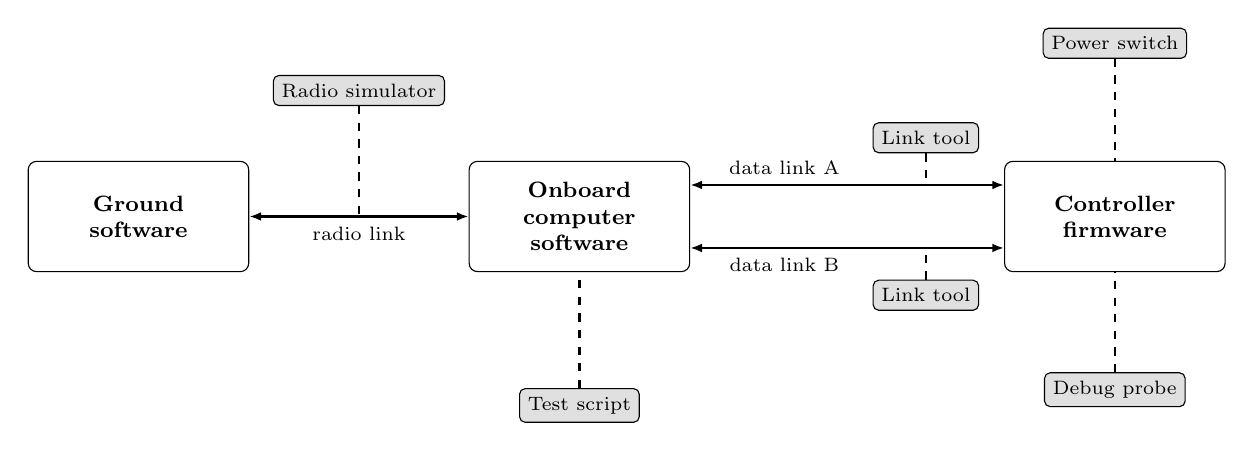
\begin{tikzpicture}[font=\scriptsize,
  item/.style={draw, rounded corners=3pt, minimum width=2.8cm, minimum height=1.4cm, align=center, font=\footnotesize\bfseries},
  tool/.style={draw, fill=black!12, rounded corners=2pt, align=center, inner sep=3pt, execute at begin node=\nohyph},
  ar/.style={{Latex[length=1.5mm]}-{Latex[length=1.5mm]}, thick},
  tl/.style={dashed, thick}]
\node[item] (g) at (0,0) {Ground\\software};
\node[item] (o) at (5.6,0) {Onboard\\computer\\software};
\node[item] (c) at (12.4,0) {Controller\\firmware};
\node[tool] (rs) at (2.8,1.6) {Radio simulator};
\node[tool] (la) at (10.0,1.0) {Link tool};
\node[tool] (lb) at (10.0,-1.0) {Link tool};
\node[tool] (ps) at (12.4,2.2) {Power switch};
\node[tool] (dp) at (12.4,-2.2) {Debug probe};
\node[tool] (ts) at (5.6,-2.4) {Test script};
\draw[ar] (g.east) -- node[below]{radio link} (o.west);
\draw[tl] (rs) -- (2.8,0);
\draw[ar] ($(o.east)+(0,0.4)$) -- node[above, pos=0.3]{data link A} ($(c.west)+(0,0.4)$);
\draw[ar] ($(o.east)+(0,-0.4)$) -- node[below, pos=0.3]{data link B} ($(c.west)+(0,-0.4)$);
\draw[tl] (la) -- (10.0,0.4);
\draw[tl] (lb) -- (10.0,-0.4);
\draw[tl] (ps) -- (c.north);
\draw[tl] (dp) -- (c.south);
\draw[tl] (ts) -- (o.south);
\end{tikzpicture}
\caption{The bench. Grey: test tools; dashed: where each one acts. The
reprogramming links are not drawn; the debug probe shares the controller's
debug port with reprogramming link A, one at a time.}
\label{fig:setup}
\end{figure}

% ===========================================================================
\section{Verification Methods}
Each requirement is verified by the method in the ``Verified by'' column of
the requirements specification [3,~Secs.~4.0--7.0]. The four methods [1,~p.~93]:

\begin{description}
\item[Test] ``The use of an end product to obtain detailed data needed to
  verify performance or provide sufficient information to verify performance
  through further analysis.''
\item[Analysis] ``The use of mathematical modeling and analytical techniques
  to predict the suitability of a design to stakeholder expectations based on
  calculated data or data derived from lower system structure end product
  verifications.''
\item[Inspection] ``The visual examination of a realized end product.''
  It ``can include inspection of drawings, documents, or other records.''
\item[Demonstration] ``Showing that the use of an end product achieves the
  individual specified requirement.''
\end{description}

\noindent Tests and demonstrations run at one of four levels:

\begin{description}[leftmargin=3.8cm]
\item[COMPONENT] One component of the architecture [5,~Sec.~6.0] alone; test
  code stands in for its neighbours.
\item[ITEM] One software item alone; test tools stand in for its neighbours.
\item[INTEGRATION] Two or more items together, over their real interfaces.
\item[SYSTEM] All three items together, with faults caused on purpose.
\end{description}

% ===========================================================================
\section{Test Articles}
The test articles are breadboards: ``a low fidelity unit that demonstrates
function only'', which ``often uses commercial and/or ad hoc components and is
not intended to provide definitive information regarding operational
performance'' [1,~p.~124]. Besides the hardware needs of the architecture
[5,~Sec.~8.0], the bench must let the test tools do the following:

\begin{enumerate}
\item Cut and restore each data link on command, and change bytes on it.
\item Cut the controller's power at a chosen moment, including during a write
  to its memory.
\item Restart the onboard computer, and stop any of its programs.
\item Read and change the controller's memory without its software, sharing
  the debug port with the onboard computer one at a time.
\item Time-stamp events on every unit from one clock.
\item Open and close contact windows, and drop, repeat, change or forge
  messages on the radio link.
\end{enumerate}

\noindent The hardware is chosen in a trade study against these needs and the
hardware needs of the architecture, and is named here \tbd{hardware}.

% ===========================================================================
\section{Component and Item Verification}
Each component, then each software item, is tested alone. A test passes when
its success criterion holds in every run. Each activity is broken into test
procedures, one per condition, once the test articles are chosen
[2,~SWE-065, Sec.~4.5.2, p.~35]. The activities of the three software items run
at the ITEM level.

\subsection{Components}
Every component of the architecture is tested alone, at the COMPONENT level
[2,~SWE\mbox{-}062, Sec.~4.4.5, p.~34]. Its tests are written with its code, and its
results are repeatable [2,~SWE\mbox{-}186, Sec.~4.4.6, p.~35]. The safety-critical
components reach 100\,\% modified condition/decision coverage [3,~REQ-108].
The test cases are kept with the code, not listed in this plan.

\subsection{Controller Firmware}

\subsection{Controller Firmware}
% BEGIN GENERATED ctl
{\footnotesize
\begin{xltabular}{\textwidth}{@{}>{\raggedright\arraybackslash}p{3.0cm}>{\raggedright\arraybackslash}X>{\raggedright\arraybackslash}p{2.4cm}@{}}
\toprule
Activity & Success criterion & Requirements \\
\midrule
\endhead
\textbf{Test-1}\newline Modes & Every transition of the ConOps mode table is driven. The controller reports exactly one mode at all times, accepts each command only in the modes that allow it, and makes no other transition. & REQ-001 to 003 \\
\textbf{Test-2}\newline Safe state & After every start, and after every function that ends, the outputs are in the safe state before any command acts. A safe-state command reaches the safe state from every mode. & REQ-004, REQ-102, REQ-106 \\
\textbf{Test-3}\newline Image checks & An image with one bit changed, or with either signature invalid, is not run, and the current copy keeps running. & REQ-005, REQ-006 \\
\textbf{Test-4}\newline Trial & New firmware runs a trial of the set length and is confirmed only when judged good. It is given up, and the previous copy runs, when not judged good in time, when it hangs, or on the operator's order. The switch happens at the set moment. & REQ-011 to 014, REQ-020, REQ-021, REQ-113 \\
\textbf{Test-5}\newline Failed starts & After the set number of failed starts, power cuts during a trial included, the previous copy runs. The count survives restarts and power cuts. Failed firmware is not started again unless ordered. & REQ-015 to 017, REQ-019 \\
\textbf{Test-6}\newline Fall-back & An update never changes the previous copy or the last-resort firmware, checked by reading memory back. When the previous copy also fails, the last-resort firmware runs, receives new firmware, and stays in FALLBACK until the operator acts. & REQ-007, REQ-008, REQ-010, REQ-018, REQ-117 \\
\textbf{Test-7}\newline Restart & Firmware made to hang restarts on its own within the restart time and resumes operation. & REQ-022, REQ-023 \\
\textbf{Test-8}\newline Independence & The controller keeps working while the onboard computer restarts, with both data links cut, and through a run of \tbd{runlen} without commands. & REQ-024 to 026 \\
\textbf{Test-9}\newline Command checks & Each command not allowed in the mode, with impossible values, not armed, armed too long ago, past its expiry, or scheduled while the clocks disagree is refused with its reason. A command sent again runs once and is answered ALREADY DONE. A held command changed before its run time is refused. No single changed bit of the stored arm state arms it. & REQ-027 to 032, REQ-133, REQ-134, REQ-137 \\
\textbf{Test-10}\newline Answers & Every command gets RECEIVED, then DONE only after its effect is seen, or REFUSED with its reason. & REQ-033 to 035 \\
\textbf{Test-11}\newline Reports and faults & Health reports arrive at the set rate. Each injected fault, failed self-test and fall-back produces its event report. A changed bit in the controller's memory is detected and leads to the safe state. Traffic from the controller never stops the onboard computer reaching it. & REQ-037 to 042 \\
\textbf{Test-12}\newline Clock & With the onboard computer's clock stopped or wrong, the controller's clock keeps time from its own source and changes only on SET CONTROLLER TIME. Every report carries both times. & REQ-131, REQ-132, REQ-135 \\
\bottomrule
\end{xltabular}}
\addtocounter{table}{-1}
% END GENERATED ctl

\subsection{Onboard Computer Software}
% BEGIN GENERATED obc
{\footnotesize
\begin{xltabular}{\textwidth}{@{}>{\raggedright\arraybackslash}p{3.0cm}>{\raggedright\arraybackslash}X>{\raggedright\arraybackslash}p{2.4cm}@{}}
\toprule
Activity & Success criterion & Requirements \\
\midrule
\endhead
\textbf{Test-13}\newline Image checks & Images not released by the operator, damaged, older than the minimum version, or built for another controller are refused with their reason. An image changed after its last transfer is refused before delivery. & REQ-043 to 047 \\
\textbf{Test-14}\newline Upload and delivery & An upload cut at random chunks resumes where it stopped. Delivery runs while the controller works. Delivery during a trial is refused with its reason. A cancelled update leaves the working firmware running and frees the storage. & REQ-048 to 052 \\
\textbf{Test-15}\newline Limits & SET LIMITS changes the minimum version and the controller identity, and only after an arming command. & REQ-053 \\
\textbf{Test-16}\newline Command intake & Frames not encrypted with the right key, with either signature invalid, sent again, or past their expiry are refused and logged. Commands that do not arrive over the radio link are refused. A dangerous command without a valid arming command is not passed on. & REQ-064 to 067, REQ-112, REQ-127, REQ-129 \\
\textbf{Test-17}\newline Scheduled commands & A scheduled command is passed on at its run time, once, also across a restart and a power cut. A held command with a changed bit is not passed on. & REQ-068, REQ-069, REQ-136 \\
\textbf{Test-18}\newline Report store & Every report is numbered, time-tagged, checked on arrival, kept through power cuts and restarts, and sent at the next contact, events first. When storage fills, the oldest health reports go first, and the number and time span dropped are reported. A clock difference above the limit is reported, and a correction of the onboard clock that does not rely on it is accepted. & REQ-070 to 079 \\
\textbf{Test-19}\newline Data links & With either data link cut, all traffic continues on the other. Each loss and each recovery is reported. With both cut, the reprogramming link still works. & REQ-080 to 083 \\
\textbf{Test-20}\newline Key replacement & A new key is accepted only in a command proven with the current one. Afterwards only the new key works. A replacement cut at any step leaves the current key working. & REQ-084 to 086 \\
\textbf{Test-21}\newline Command log & The ground receives a log of every command acted on, including one injected past the ground. & REQ-087 \\
\textbf{Test-22}\newline Recovery & A silent controller is noticed and brought back, and the attempt is recorded. After a program is killed, and after the whole onboard computer restarts, the update in progress resumes. & REQ-061 to 063 \\
\bottomrule
\end{xltabular}}
\addtocounter{table}{-1}
% END GENERATED obc

\subsection{Ground Software}
% BEGIN GENERATED gnd
{\footnotesize
\begin{xltabular}{\textwidth}{@{}>{\raggedright\arraybackslash}p{3.0cm}>{\raggedright\arraybackslash}X>{\raggedright\arraybackslash}p{2.4cm}@{}}
\toprule
Activity & Success criterion & Requirements \\
\midrule
\endhead
\textbf{Test-23}\newline Ground checks & Every command and release leaves signed twice. Malformed commands, and releases for another controller, older than the minimum version or not the tested build, are not sent. Each signed image passes the onboard computer's checks before it is sent. A planned sequence stops at the first refusal or missing answer. & REQ-088 to 090, REQ-114 to 116 \\
\textbf{Test-24}\newline Ground display & A damaged report is marked on arrival. Every command still waiting for its answers, and the running firmware, are shown. & REQ-093 to 095 \\
\textbf{Demonstration-1}\newline Operator access & Someone without the operator's credentials cannot use the operator interface. & REQ-091 \\
\textbf{Demonstration-2}\newline Planning & The operator plans commands, uploads and report retrieval for coming contacts. & REQ-097 \\
\bottomrule
\end{xltabular}}
\addtocounter{table}{-1}
% END GENERATED gnd

% ===========================================================================
\section{System Verification}
The items are then verified together. The restore and the interfaces are
verified at the INTEGRATION level; fault injection and scenario runs at the
SYSTEM level.

\subsection{Restore}
% BEGIN GENERATED rst
{\footnotesize
\begin{xltabular}{\textwidth}{@{}>{\raggedright\arraybackslash}p{3.0cm}>{\raggedright\arraybackslash}X>{\raggedright\arraybackslash}p{2.4cm}@{}}
\toprule
Activity & Success criterion & Requirements \\
\midrule
\endhead
\textbf{Test-25}\newline Restore & With the controller's memory erased, and with its bootloader damaged, a restore through each reprogramming link writes only checked images, puts the last-resort firmware first and clears the kept data. On order, it puts back the bootloader and the main firmware. The onboard computer restarts the controller, checks its copy and the links between uses, and tells the ground the result. & REQ-054, REQ-057 to 060, REQ-118, REQ-120 to 122, REQ-124 \\
\textbf{Demonstration-3}\newline Restore on order & The operator orders a restore while firmware runs, and it completes. & REQ-055 \\
\bottomrule
\end{xltabular}}
\addtocounter{table}{-1}
% END GENERATED rst

\subsection{Interfaces}
% BEGIN GENERATED ifc
{\footnotesize
\begin{xltabular}{\textwidth}{@{}>{\raggedright\arraybackslash}p{3.0cm}>{\raggedright\arraybackslash}X>{\raggedright\arraybackslash}p{2.4cm}@{}}
\toprule
Activity & Success criterion & Requirements \\
\midrule
\endhead
\textbf{Test-26}\newline Interfaces & Every message on each interface matches the Interface Design byte for byte. A frame with any byte changed is dropped on every link. & REQ-107 \\
\bottomrule
\end{xltabular}}
\addtocounter{table}{-1}
% END GENERATED ifc

\subsection{Fault Injection}
% BEGIN GENERATED flt
{\footnotesize
\begin{xltabular}{\textwidth}{@{}>{\raggedright\arraybackslash}p{3.0cm}>{\raggedright\arraybackslash}X>{\raggedright\arraybackslash}p{2.4cm}@{}}
\toprule
Activity & Success criterion & Requirements \\
\midrule
\endhead
\textbf{Test-27}\newline Fault injection & Each fault of Table~\ref{tab:faults} is injected during operation. Every detected error is handled, the response matches the ConOps scenario, and no hazard occurs. & REQ-105 \\
\bottomrule
\end{xltabular}}
\addtocounter{table}{-1}
% END GENERATED flt

\begin{table}[H]
\centering
{\small\begin{tabularx}{\textwidth}{@{}>{\raggedright\arraybackslash}Xll@{}}
\toprule
Fault & Caused by & ConOps scenario \\
\midrule
Radio link cut during an upload & RADIO SIMULATOR & Scenario-200 \\
Long gap between contacts fills the report storage & RADIO SIMULATOR & Scenario-210 \\
Forged command, or old command sent again & RADIO SIMULATOR & Scenario-300 \\
Firmware damaged in transfer & RADIO SIMULATOR & Scenario-400 \\
New firmware hangs, restarts over and over, or is never judged good & TEST FIRMWARE & Scenario-430 to 450 \\
Previous firmware also unusable & DEBUG PROBE & Scenario-460 \\
No firmware can run & DEBUG PROBE & Scenario-480 \\
One data link cut, then restored; both cut & LINK TOOL & Scenario-500 to 510 \\
Controller goes silent & DEBUG PROBE & Scenario-520 \\
Program on the onboard computer stopped & TEST SCRIPT & Scenario-530 \\
Whole onboard computer restarted & TEST SCRIPT & Scenario-535 \\
Power cut during a firmware write, and during a trial & POWER SWITCH & Scenario-600, 605 \\
Bit changed in stored firmware & DEBUG PROBE & Scenario-610 \\
Bit changed in the memory the controller runs from & DEBUG PROBE & Scenario-620 \\
\bottomrule
\end{tabularx}}
\caption{Faults caused on purpose [4,~Sec.~6.2].}
\label{tab:faults}
\end{table}

\subsection{Scenario Runs}
% BEGIN GENERATED scn
{\footnotesize
\begin{xltabular}{\textwidth}{@{}>{\raggedright\arraybackslash}p{3.0cm}>{\raggedright\arraybackslash}X>{\raggedright\arraybackslash}p{2.4cm}@{}}
\toprule
Activity & Success criterion & Requirements \\
\midrule
\endhead
\textbf{Test-28}\newline Scenario runs & Every ConOps scenario, nominal and off-nominal, is run from start to end, and each shows the outcome the ConOps states. & --- \\
\bottomrule
\end{xltabular}}
\addtocounter{table}{-1}
% END GENERATED scn

\subsection{Inspections and Analyses}
% BEGIN GENERATED ins
{\footnotesize
\begin{xltabular}{\textwidth}{@{}>{\raggedright\arraybackslash}p{3.0cm}>{\raggedright\arraybackslash}X>{\raggedright\arraybackslash}p{2.4cm}@{}}
\toprule
Activity & Success criterion & Requirements \\
\midrule
\endhead
\textbf{Inspection-1}\newline Separate code & The link maps and source lists of the parts each requirement keeps apart share no file, library or symbol. & REQ-009, REQ-099, REQ-119, REQ-123, REQ-126, REQ-130 \\
\textbf{Inspection-2}\newline Records & The test logs hold every command received and answer sent. The ground archive holds every report sent. The recoverable copy of the keys restores them. & REQ-036, REQ-092, REQ-096 \\
\textbf{Inspection-3}\newline Shared list & The ground and the onboard software take their commands and refusal reasons from one source file. & REQ-100 \\
\textbf{Inspection-4}\newline Operating builds & The operating builds contain no fault-injection function. & REQ-101 \\
\textbf{Inspection-5}\newline Code rules & Tool reports show a complexity of 15 or lower for each safety-critical component, conformance to the coding standard, and no open static-analysis finding. & REQ-109 to 111 \\
\textbf{Inspection-6}\newline Ways back in & No controller firmware writes the option bytes or the boot settings, and the factory loader driver never sends Readout Protect or Write Protect. & REQ-125 \\
\textbf{Inspection-7}\newline Keys and links & The two signing keys and the encryption key are kept in three separate places. The two data links are of different kinds. & REQ-128, REQ-138 \\
\textbf{Analysis-1}\newline Fault tolerance & The hazard analysis, run again on the built System, finds at least three failures for each catastrophic hazard and two for each critical one, the accepted exceptions aside, and no hazard started by a single software event. & REQ-098, REQ-103 \\
\textbf{Analysis-2}\newline Response times & For each off-nominal condition, the response time measured in Test-27 is shorter than the time to the hazard. & REQ-104 \\
\textbf{Analysis-3}\newline Restore independence & The restore sequences of the Interface Design use no controller software: the core is held stopped, or the factory loader runs from read-only memory. & REQ-056 \\
\textbf{Analysis-4}\newline Coverage & The coverage tool reports 100\,\% modified condition/decision coverage of the safety-critical software over all tests. & REQ-108 \\
\bottomrule
\end{xltabular}}
\addtocounter{table}{-1}
% END GENERATED ins

\subsection{Hardware}
These two activities check the hardware itself, against the hardware needs of
the architecture [5,~Sec.~8.0] and of Section~5.0. They run once the hardware
is chosen.
% BEGIN GENERATED hw
{\footnotesize
\begin{xltabular}{\textwidth}{@{}>{\raggedright\arraybackslash}p{3.0cm}>{\raggedright\arraybackslash}X>{\raggedright\arraybackslash}p{2.4cm}@{}}
\toprule
Activity & Success criterion & Needs \\
\midrule
\endhead
\textbf{Inspection-8}\newline Hardware documents & Every hardware need of the architecture, and every need of Section~5.0, is shown met by the chosen hardware's datasheets and manuals, each with its page. & Architecture Section~8.0; Section~5.0 \\
\textbf{Test-29}\newline Hardware measurements & The needs that documents cannot settle are measured on the test articles: two signatures are checked at start-up within the restart time of REQ-023; software cannot stop the watchdog; the clock runs from its own source, at a measured rate; the debug port and the factory loader reach all of memory with the controller held in reset. & Architecture Section~8.0 \\
\bottomrule
\end{xltabular}}
\addtocounter{table}{-1}
% END GENERATED hw

% ===========================================================================
\section{Limits of Bench Verification}
The System runs on commercial development boards: ``It can show how the System
behaves, not that it would survive launch or space'' [4,~Sec.~1.1.2]. The
requirements below are verified only in part. What the bench cannot show is
the risk left, accepted by the author.

\smallskip
{\small\noindent\begin{tabularx}{\textwidth}{@{}l>{\raggedright\arraybackslash}X>{\raggedright\arraybackslash}X@{}}
\toprule
Requirement & The bench shows & The bench cannot show \\
\midrule
REQ-041 & A bit changed on purpose is detected & Real radiation: its rate, several bits changed at once, damage to the chip \\
REQ-026 & Correct operation through the run of Test-8 & Operation for longer than that run \\
REQ-064, REQ-129 & Forged and changed frames are refused & Resistance to every possible forgery, which rests on Ed25519 and AES-256 in Galois/Counter Mode \\
REQ-098, REQ-103 & Nothing; Analysis-1 shows it & That the analysis found every combination of failures \\
REQ-080 & Both data links work over bench cables & The length and electrical noise of a spacecraft harness \\
REQ-067 & Contact windows and losses made by the radio simulator & The real radio equipment, which lies outside the System \\
All & Behaviour at room temperature and pressure & Temperature, vacuum, vibration and launch \\
\bottomrule
\end{tabularx}}

% ===========================================================================
\appendix
\renewcommand{\thesection}{\Alph{section}}
\renewcommand{\thesubsection}{\Alph{section}.\arabic{subsection}}

\section{Verification Matrix}
Each requirement, its verification method [3,~Secs.~4.0--7.0], and the
activities that verify it [1,~App.~D, p.~201].

% BEGIN GENERATED matrix
{\scriptsize
\begin{xltabular}{\textwidth}{@{}lll@{\hspace{1.2em}}lll@{}}
\toprule
Req. & Method & Activities & Req. & Method & Activities \\
\midrule
\endhead
REQ-001 & TEST & Test-1 & REQ-070 & TEST & Test-18 \\
REQ-002 & TEST & Test-1 & REQ-071 & TEST & Test-18 \\
REQ-003 & TEST & Test-1 & REQ-072 & TEST & Test-18 \\
REQ-004 & TEST & Test-2 & REQ-073 & TEST & Test-18 \\
REQ-005 & TEST & Test-3 & REQ-074 & TEST & Test-18 \\
REQ-006 & TEST & Test-3 & REQ-075 & TEST & Test-18 \\
REQ-007 & TEST & Test-6 & REQ-076 & TEST & Test-18 \\
REQ-008 & TEST & Test-6 & REQ-077 & TEST & Test-18 \\
REQ-009 & INSPECTION & Inspection-1 & REQ-078 & TEST & Test-18 \\
REQ-010 & TEST & Test-6 & REQ-079 & TEST & Test-18 \\
REQ-011 & TEST & Test-4 & REQ-080 & TEST & Test-19 \\
REQ-012 & TEST & Test-4 & REQ-081 & TEST & Test-19 \\
REQ-013 & TEST & Test-4 & REQ-082 & TEST & Test-19 \\
REQ-014 & TEST & Test-4 & REQ-083 & TEST & Test-19 \\
REQ-015 & TEST & Test-5 & REQ-084 & TEST & Test-20 \\
REQ-016 & TEST & Test-5 & REQ-085 & TEST & Test-20 \\
REQ-017 & TEST & Test-5 & REQ-086 & TEST & Test-20 \\
REQ-018 & TEST & Test-6 & REQ-087 & TEST & Test-21 \\
REQ-019 & TEST & Test-5 & REQ-088 & TEST & Test-23 \\
REQ-020 & TEST & Test-4 & REQ-089 & TEST & Test-23 \\
REQ-021 & TEST & Test-4 & REQ-090 & TEST & Test-23 \\
REQ-022 & TEST & Test-7 & REQ-091 & DEMONSTRATION & Demonstration-1 \\
REQ-023 & TEST & Test-7 & REQ-092 & INSPECTION & Inspection-2 \\
REQ-024 & TEST & Test-8 & REQ-093 & TEST & Test-24 \\
REQ-025 & TEST & Test-8 & REQ-094 & TEST & Test-24 \\
REQ-026 & TEST & Test-8 & REQ-095 & TEST & Test-24 \\
REQ-027 & TEST & Test-9 & REQ-096 & INSPECTION & Inspection-2 \\
REQ-028 & TEST & Test-9 & REQ-097 & DEMONSTRATION & Demonstration-2 \\
REQ-029 & TEST & Test-9 & REQ-098 & ANALYSIS & Analysis-1 \\
REQ-030 & TEST & Test-9 & REQ-099 & INSPECTION & Inspection-1 \\
REQ-031 & TEST & Test-9 & REQ-100 & INSPECTION & Inspection-3 \\
REQ-032 & TEST & Test-9 & REQ-101 & INSPECTION & Inspection-4 \\
REQ-033 & TEST & Test-10 & REQ-102 & TEST & Test-2 \\
REQ-034 & TEST & Test-10 & REQ-103 & ANALYSIS & Analysis-1 \\
REQ-035 & TEST & Test-10 & REQ-104 & ANALYSIS & Analysis-2 \\
REQ-036 & INSPECTION & Inspection-2 & REQ-105 & TEST & Test-27 \\
REQ-037 & TEST & Test-11 & REQ-106 & TEST & Test-2 \\
REQ-038 & TEST & Test-11 & REQ-107 & TEST & Test-26 \\
REQ-039 & TEST & Test-11 & REQ-108 & ANALYSIS & Analysis-4 \\
REQ-040 & TEST & Test-11 & REQ-109 & INSPECTION & Inspection-5 \\
REQ-041 & TEST & Test-11 & REQ-110 & INSPECTION & Inspection-5 \\
REQ-042 & TEST & Test-11 & REQ-111 & INSPECTION & Inspection-5 \\
REQ-043 & TEST & Test-13 & REQ-112 & TEST & Test-16 \\
REQ-044 & TEST & Test-13 & REQ-113 & TEST & Test-4 \\
REQ-045 & TEST & Test-13 & REQ-114 & TEST & Test-23 \\
REQ-046 & TEST & Test-13 & REQ-115 & TEST & Test-23 \\
REQ-047 & TEST & Test-13 & REQ-116 & TEST & Test-23 \\
REQ-048 & TEST & Test-14 & REQ-117 & TEST & Test-6 \\
REQ-049 & TEST & Test-14 & REQ-118 & TEST & Test-25 \\
REQ-050 & TEST & Test-14 & REQ-119 & INSPECTION & Inspection-1 \\
REQ-051 & TEST & Test-14 & REQ-120 & TEST & Test-25 \\
REQ-052 & TEST & Test-14 & REQ-121 & TEST & Test-25 \\
REQ-053 & TEST & Test-15 & REQ-122 & TEST & Test-25 \\
REQ-054 & TEST & Test-25 & REQ-123 & INSPECTION & Inspection-1 \\
REQ-055 & DEMONSTRATION & Demonstration-3 & REQ-124 & TEST & Test-25 \\
REQ-056 & ANALYSIS & Analysis-3 & REQ-125 & INSPECTION & Inspection-6 \\
REQ-057 & TEST & Test-25 & REQ-126 & INSPECTION & Inspection-1 \\
REQ-058 & TEST & Test-25 & REQ-127 & TEST & Test-16 \\
REQ-059 & TEST & Test-25 & REQ-128 & INSPECTION & Inspection-7 \\
REQ-060 & TEST & Test-25 & REQ-129 & TEST & Test-16 \\
REQ-061 & TEST & Test-22 & REQ-130 & INSPECTION & Inspection-1 \\
REQ-062 & TEST & Test-22 & REQ-131 & TEST & Test-12 \\
REQ-063 & TEST & Test-22 & REQ-132 & TEST & Test-12 \\
REQ-064 & TEST & Test-16 & REQ-133 & TEST & Test-9 \\
REQ-065 & TEST & Test-16 & REQ-134 & TEST & Test-9 \\
REQ-066 & TEST & Test-16 & REQ-135 & TEST & Test-12 \\
REQ-067 & TEST & Test-16 & REQ-136 & TEST & Test-17 \\
REQ-068 & TEST & Test-17 & REQ-137 & TEST & Test-9 \\
REQ-069 & TEST & Test-17 & REQ-138 & INSPECTION & Inspection-7 \\
\bottomrule
\end{xltabular}}
\addtocounter{table}{-1}
% END GENERATED matrix

\section{Acronyms}
\begin{description}[leftmargin=2.2cm]
\item[ConOps] Concept of Operations
\item[TBD] To Be Determined
\item[TBR] To Be Resolved
\end{description}

\section{Open Items}
The values below are not yet known.
\begin{description}
\tbditem{ref}{Project name and document reference.}
\tbditem{runlen}{Length of the run without commands in Test-8.}
\tbditem{hardware}{The test articles, chosen in a hardware trade study
  (Section~5.0).}
\end{description}

\medskip
\noindent All statements in this document were stated or accepted by the
author on 12 October 2026.

\end{document}
